\section{Iterations}

In here will be the description of the method and results of iterating between solvings of M and C until the difference has convergenced to a a specificed epsilon. Also mention in here the effects it has on the solutions (not much) and computation time (2x longer ish?). Also discuss the single iterations and its effects (solve M -> solve C -> solve M again).


  The system
  \begin{align}
    M_t &= \nabla_x \left( D(M) \nabla_x M \right) + f(C,M) M \\
    C_t &= - g(C,M) 
  \end{align}
  where
  \begin{align}
    D(M) &= \delta \frac{M^\alpha}{(1 - M)^\beta} \\
    f(C,M) &= \frac{ C }{{k } + {C}} \left(1 - \left( \frac{M M_0}{{C C_0 + \epsilon}} \right)^\gamma \right) \\
    g(C,M) &= \frac{\nu C}{k +C} M
  \end{align}
  is solved on a rectangular region with length $L$ and width $\lambda L$ with the following parameter values,
  \begin{equation}
    \begin{aligned}
      L &= 0.01 \\
      \lambda &= \frac{1}{128}\\
      \epsilon &= 10^{-8}\\
      \alpha &= 4 \\
      \beta &= 4 \\
      \gamma &= 0.5 \\
      \mu &= 6 \\      
    \end{aligned}
    \qquad
    \begin{aligned}
      C_0 &= 30 \\
      M_0 &= 30 \\
      \delta &= \frac{10^{-7}}{\mu L^2} \approx 10^-4\\
      k &= \frac{4}{C_0} \approx 0.1333\\
      \nu &= \frac{M_0}{0.63 C_0} \approx 1.59,\\
    \end{aligned}
  \end{equation}
  and with initial conditions 
  \begin{equation}
    \begin{aligned}
      C &= 1 \\
      M &= \begin{cases} -(\frac{h}{d^4})x^4 + h & \text{if } x < 0.04 \\ 0 & \text{otherwise }\end{cases} \\
    \end{aligned}
  \end{equation}  
  where $h = 0.1, d=\frac{5}{128}$ , representing the height and depth of the inoculation site.

  Using simulation code version $0.4$ the effect of iterating between solving $M$ and $C$ was examined. Algorithm \ref{alg:iterateCM} shows how the iterations was implemented. The following experiments were run on the simulator.
  
  \begin{algorithm}[h!tb]
      \dontprintsemicolon
      \KwData{eSoln = $10^{-12}$; $M_{prev}$ and $C_{prev}$ is previous timestep solutions}
      \Begin
      {
        \SetLine
        \While{diffC + diffM  $> $ eSoln}
        {
            Solve for $M^{i+1}$ using $C^{i}$ and $M_{prev}$\;
            Solve for $C^{i+1}$ using $C_{prev}$, $M^{i+1}$, and $M_{prev}$\;
            Let diffC $=  (C^{i+1} - C^i)$\;
            Let diffM $= (M^{i+1} - M^i)$\;
            Let $C^{i} = C^{i+1}$\;
            Let $M^{i} = M^{i+1}$\;
        }
      }
      \caption{Algorithm for iterating between solutions.}
      \label{alg:iterateCM}
    \end{algorithm}
  
  Figure \ref{fig:iterateAccuracy} shows how the error between the iterated solutions changes the solutions. Notice that there is very little difference.
  
  \begin{figure}[h!tb]
    \begin{center}
      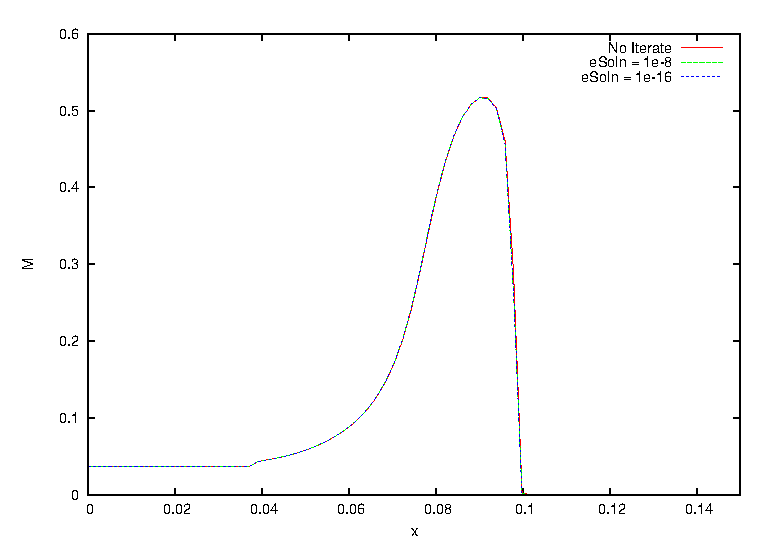
\includegraphics[scale=0.85]{eSolnCheck.eps}
      \caption{Convergence of solutions for no iterations between solutions, or iterating with different accuracy values.}
      \label{fig:iterateAccuracy}
    \end{center}
  \end{figure}
  
    
  Figure \ref{fig:convergeDelt} shows, for different $\Delta t$ values, the convergence of solutions as $\Delta x$ becomes smaller. Very minute differences between $\Delta t$ values.
  
  \begin{figure}[h!tb]
    \begin{center}
      \begin{tabular}{c c}
          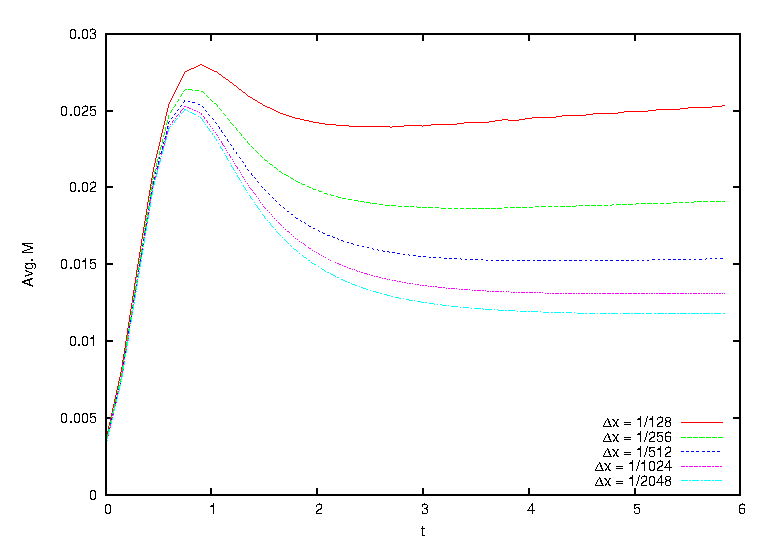
\includegraphics[scale=0.55]{converge_tDel1e-2.eps} &
          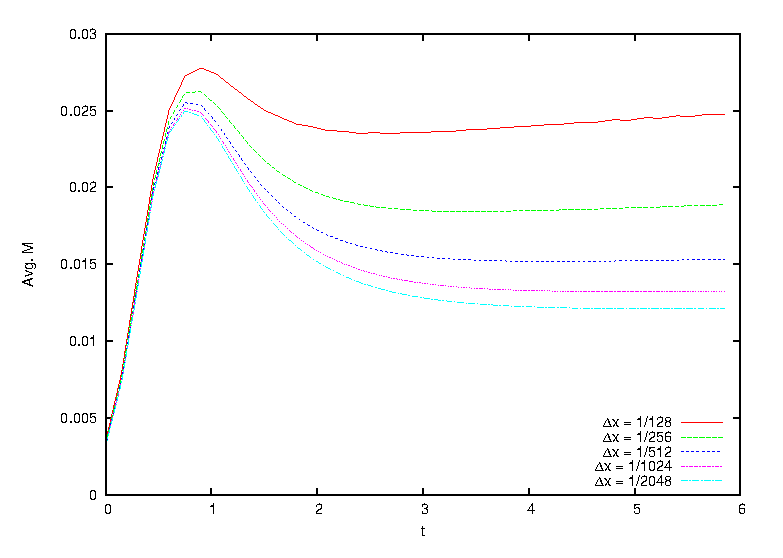
\includegraphics[scale=0.55]{converge_tDel1e-3.eps} \\
          (a) & (b) \\
          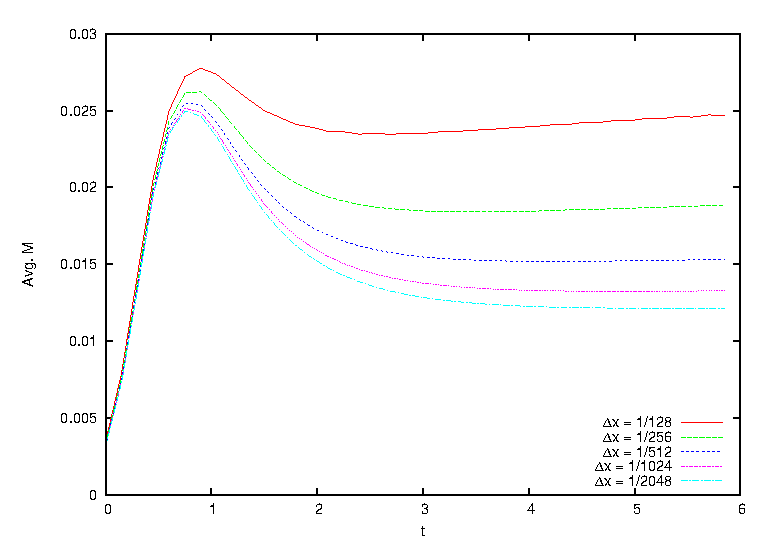
\includegraphics[scale=0.55]{converge_tDel1e-4.eps} & \\
          %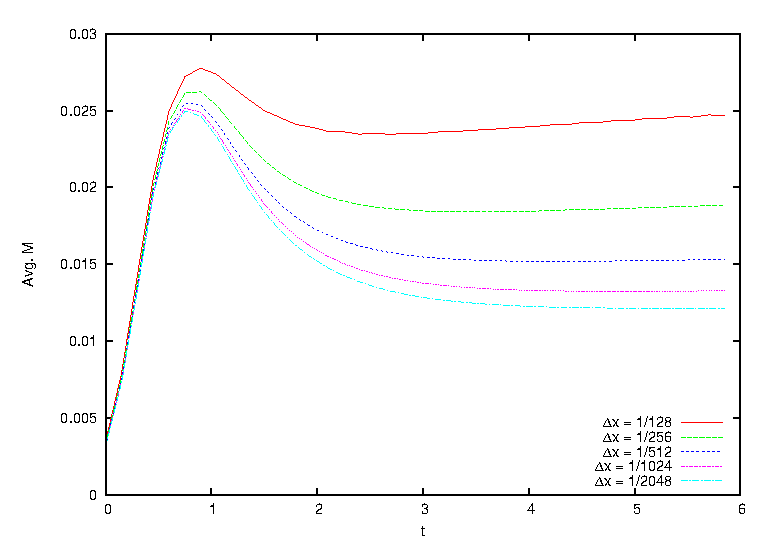
\includegraphics[scale=0.8]{converge_tDel1e-4.eps} \\
          (c) & (d)
      \end{tabular}
      \caption{Convergence of solutions for (a) $\Delta t = 10^{-2}$, (b) $\Delta t = 10^{-3}$, (c) $\Delta t = 10^{-4}$, (d) $\Delta t = 10^{-5}$.}
      \label{fig:convergeDelt}
    \end{center}
  \end{figure}
  
   Figure \ref{fig:functionC} shows the convergence of solutions if the computation of $M$ depends on a arbitrary function, $\hat{C}$, instead of the substrait concentration. 
  
  \begin{figure}[h!tb]
    \begin{center}
      \begin{tabular}{c c}
          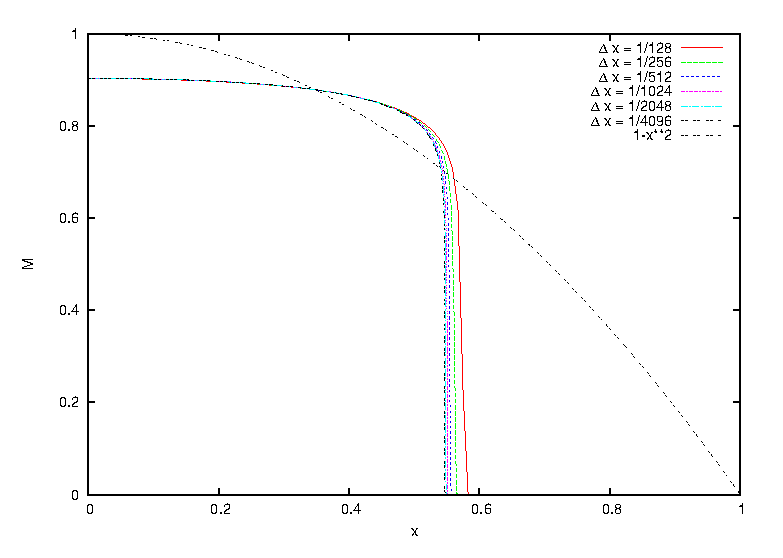
\includegraphics[scale=0.55]{Cfunc_polynomial_t=5-25.eps} &
          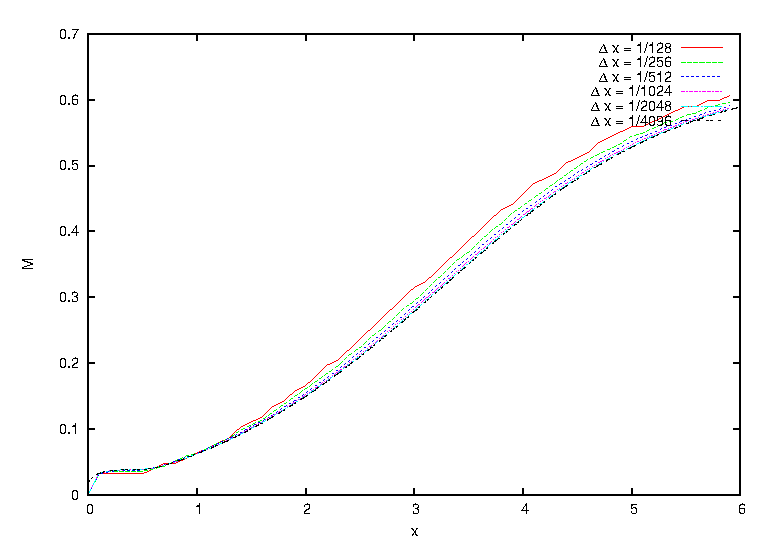
\includegraphics[scale=0.55]{Cfunc_polynomial_interface.eps} \\
          (a) & (b) 
      \end{tabular}
      \caption{Convergence of solutions for $\hat{C}(x) = 1-x^2$ looking at (a) solutions at $t = 5.25$ and (b) the interface x position.}
      \label{fig:functionC}
    \end{center}
  \end{figure}
  
   Figure \ref{fig:kinematics} show how the solutions converge for different functions $f(C,M)$. Some of which do not depend on $C$ or $M$. 
  
  \begin{figure}[h!tb]
    \begin{center}
      \begin{tabular}{c c}
          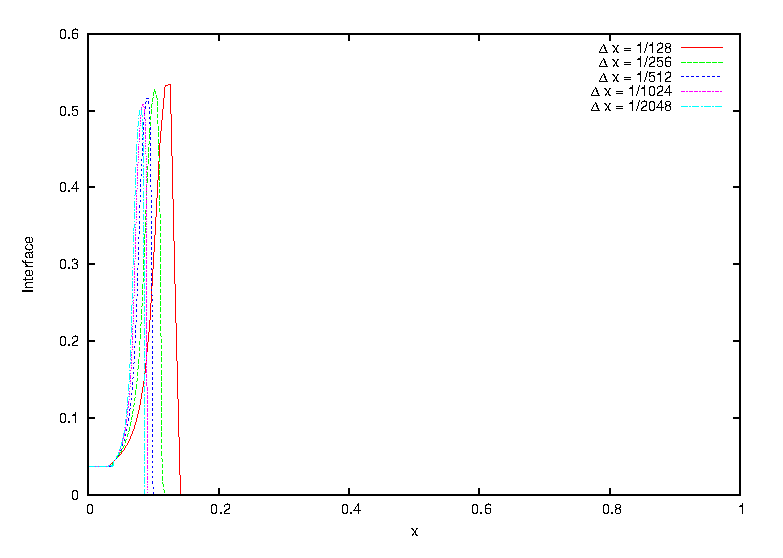
\includegraphics[scale=0.55]{Fdefault.eps} &
          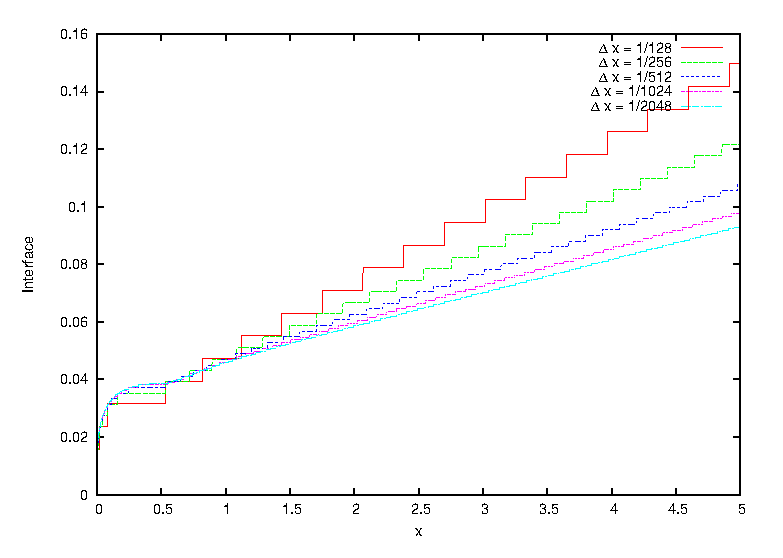
\includegraphics[scale=0.55]{FdefaultInterface.eps} \\
          (a) & (b) \\
          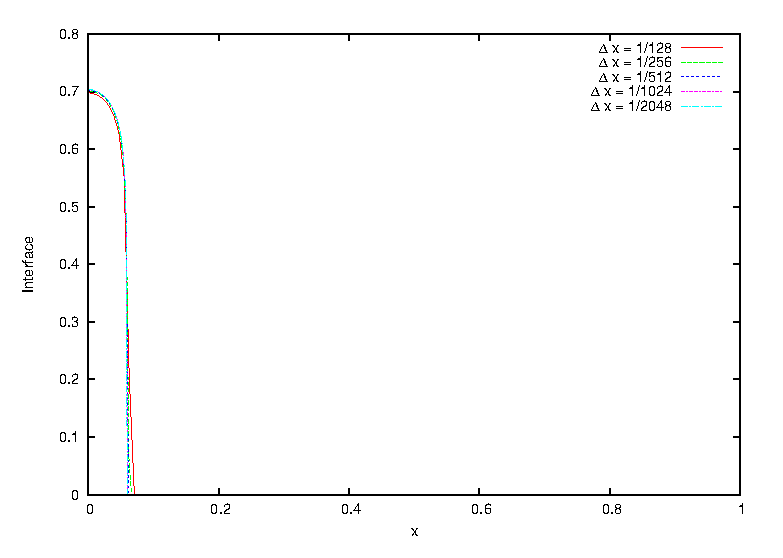
\includegraphics[scale=0.55]{Flogistic_t=4-25.eps} &
          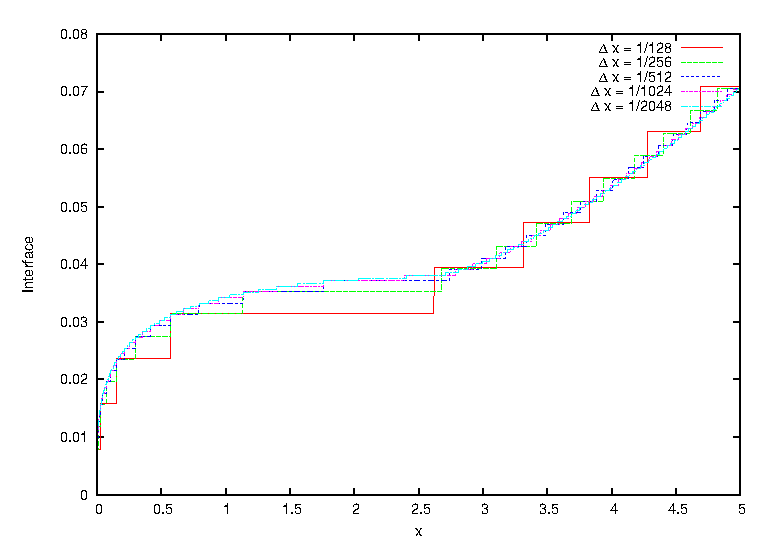
\includegraphics[scale=0.55]{Flogistic.eps} \\
          (c) & (d) \\
          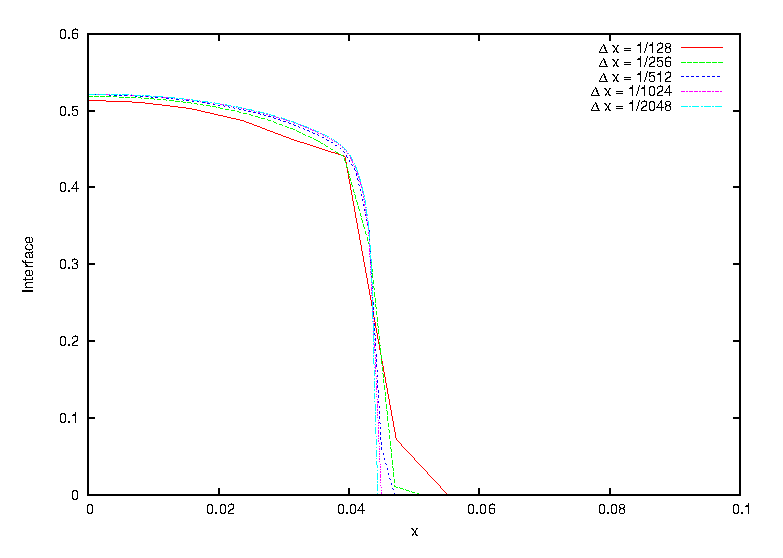
\includegraphics[scale=0.55]{FnoM.eps} &
          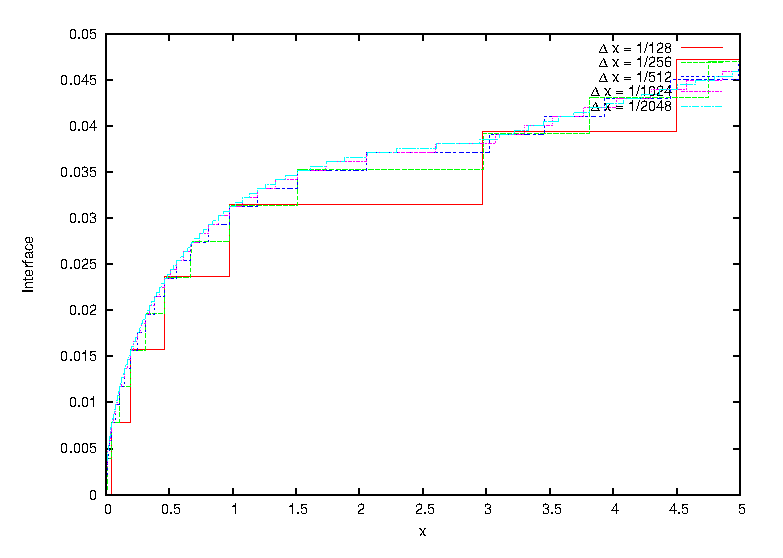
\includegraphics[scale=0.55]{FnoMInterface.eps} \\
          (e) & (f) \\
          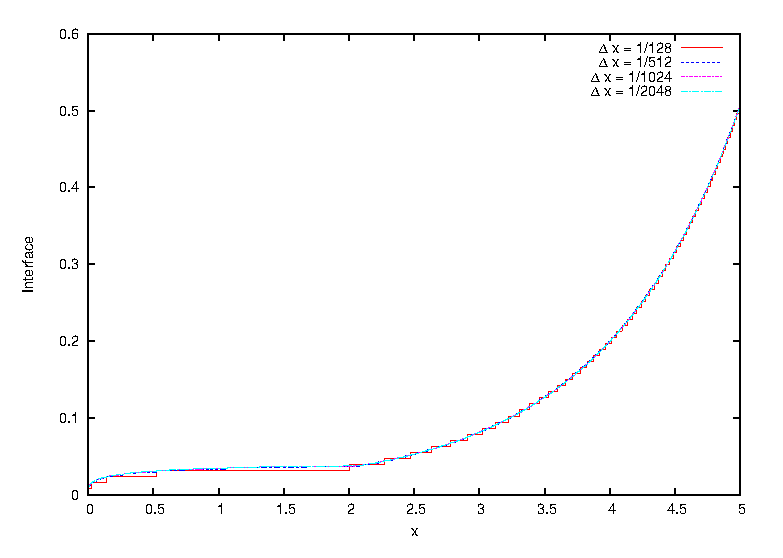
\includegraphics[scale=0.55]{Fconstant.eps} & \\
          (g) & \\ 
      \end{tabular}
      \caption{Convergence of solutions for (a-b) $f(C,M) = $default,  (c-d) $f(C,M) = (1 - M)$, (e-f) $f(C,M) = (1 - C) \frac{C}{M+\epsilon}, $(g) $f(C,M) = 1$. Each pair of graphs is the solution at $t = 4.25$ and the interface as a function of t.}
      \label{fig:kinematics}
    \end{center}
  \end{figure}


